\documentclass[12pt, letterpaper]{article}
\usepackage{graphicx}
\graphicspath{ {images/} }
% Reduce the page margins to 3/4 of an inch
\usepackage[margin=0.75in]{geometry}

\usepackage{bookmark}

\usepackage{enumitem}

% References
\usepackage{hyperref}

% Import citations for use with BibTeX
\usepackage{cite}

\usepackage[toc,page]{appendix}
% Table formatting
\usepackage{tabularx}

% Paragraph-blocks, allowing multi-line cells in tables.
\usepackage{makecell}

\usepackage{float}

% Source code
\usepackage{listings}

% Allows float barriers
\usepackage{placeins}


\newcommand{\quickfigure}[3]{
  \FloatBarrier
  \begin{figure}[!h]
    \centering
    \includegraphics[width=#1\linewidth]{#2}
    \caption{#3}
  \end{figure}
  \FloatBarrier
}

% Restrict table of contents to parts through subsubsections
\setcounter{tocdepth}{3}


\usepackage{fancyhdr}
\pagestyle{fancy}
\fancyhf{}
\newcolumntype{R}{>{\raggedleft\arraybackslash}X}%
\fancypagestyle{style1}{
\fancyhf{}
\lhead{Software Design Document}
\rhead{CIOS Digital}
\lfoot{05/16/2017}
\rfoot{\thepage}
\renewcommand{\footrulewidth}{0.4pt}
\newcolumntype{R}{>{\raggedleft\arraybackslash}X}%
}
\fancypagestyle{style2}{
\fancyhf{}
\rhead{}
\lhead{}
\cfoot{\thepage}
\renewcommand{\footrulewidth}{0.4pt}
\newcolumntype{R}{>{\raggedleft\arraybackslash}X}%
}
\pagestyle{style1}

\makeatletter
\renewcommand{\maketitle}{\bgroup\setlength{\parindent}{0pt}
\thispagestyle{empty}
\null

  \begin{flushleft}
  \vspace{15mm}
  \vskip2mm
  \Huge{\textbf{\@title}}
  \vspace{7cm}
\begin{figure}[ht]
  \begin{minipage}[b]{0.45\linewidth}
    
\includegraphics[width=.75\textwidth]{images/cios.png}
  \end{minipage}
  \hspace{0.5cm}
  \begin{minipage}[b][][c]{0.45\linewidth}
    \LARGE{\@author}
  \vspace{0.35cm}
  \end{minipage}
\end{figure}
\\CSCI 492: Spring 2017\\
  \end{flushleft}\egroup
}
\makeatother

\title{Software Requirements Specification\\for\\Flight Plan Editor}
\date{}
\author{
Cedrick Cooke\\
Ian Littke\\
Owen Roth-Lerner\\
Sander Scherman Garzon\\
}



\begin{document}
\pagenumbering{roman}
\maketitle

\newpage
\pagestyle{style2}
\setcounter{page}{1}
\section*{Revision History}
\begin{tabularx}{\textwidth}{|l|r|X|l|}
\hline
\textbf{Name} & \textbf{Date} & \textbf{Reason for Change} & \textbf{Version} \\ \hline
Various & 2017-04-13 & Initial document body and writing & Draft 1 \\ \hline
        &            &                                   &         \\ \hline
        &            &                                   &         \\ \hline
        &            &                                   &         \\ \hline
        &            &                                   &         \\ \hline
        &            &                                   &         \\ \hline
        &            &                                   &         \\ \hline
        &            &                                   &         \\ \hline
        &            &                                   &         \\ \hline
        &            &                                   &         \\ \hline
        &            &                                   &         \\ \hline
        &            &                                   &         \\ \hline
        &            &                                   &         \\ \hline
        &            &                                   &         \\ \hline
        &            &                                   &         \\ \hline
        &            &                                   &         \\ \hline
        &            &                                   &         \\ \hline
        &            &                                   &         \\ \hline
        &            &                                   &         \\ \hline
\end{tabularx}

\newpage
\tableofcontents
\newpage
\pagestyle{style1}
\pagenumbering{arabic}
\setcounter{page}{1}

\section{Introduction}
  \subsection{Purpose}
    This software design document describes the architecture and system design of the CIOS Digital Flight Planning Editor release 1.0.
    The intended audience for this document will be primarily the development team at CIOS Digital working on the Flight Planning Editor and secondary any members of the Civilian Air Patrol nationwide who will design and load flight plans to be mounted onto a Garmin G1000 equipped aircraft.

  \subsection{Scope}
    The Flight Planning Editor will allow flight planners in the Civilian Air Patrol (CAP) to plan their flights in an easy fashion and store them in a Secure Digital (SD) card. A detailed project description is available in the Flight Plan Editor Vision and Scope Document. The section in that document titled ”Scope of Initial and Subsequent Releases” lists the features that are scheduled for full or partial implementation in this release.
    This document provides the artchitecture and design of Release 1.0 of the software.

  % \subsection{Overview}
  %   Section \ref{system} of this document details the system overview and gives a description of the functionality. \\
  %   Section \ref{design} covers the system architecture including the architectural design, decomposition description, and design rationale. \\
  %   Section 4 details the data design giving a description and data dictionary. \\
  %   Section 5 is the component design, offering a comprehensive look at each component and how they link with one another. \\
  %   Section \ref{ui} includes the human interface design. \\
  %   Section 7 lists the Appendicies. \\
  \subsection{Reference Material}
    \begin{itemize}
      \setlength{\itemsep}{1pt}
      \setlength{\parskip}{0pt}
      \setlength{\parsep}{0pt}
      \item CIOS Digital Vision and Scope Document
      \item CIOS Digital Software Requirements Specification (SRS)
    \end{itemize}

  \subsection{Definitions, Acronyms, and Abbreviations}
  	\begin{tabularx}{\textwidth}{|l|R|} \hline
    	Acronym & Definition \\ \hline
    	CAP & Civilian Air Patrol  \\ \hline
    	SD & Secure Digital (Memory card) \\ \hline
  	\end{tabularx}

  \section{System Overview}\label{system}
    The CAP will need to create flight plans based on existing structures so the application will focus around a map.
    The user will then be able to either click on map to insert a new waypoint in the flight plan or manually input in a latitude/longitude coordinate system.
    Both are included to allow precise input of key waypoints (such as an overpass) or coarse input for secondary waypoints (such as an entry/depature course).
    The User Interface is furter explained in Section \ref{sec:ui}.

    %  \subsection{System context Diagram}

\section{Design Considerations} \label{dsign}
  \subsection{Assumptions and Dependencies}
    See CIOS Digital Software Requirements Specification Section 2.7 for details.
  \subsection{General Constraints}
    See CIOS Digital Software Requirements Specification Section 4 for details.
  \subsection{Goals and Guidelines}
    \begin{itemize}
      \setlength{\itemsep}{1pt}
      \setlength{\parskip}{0pt}
      \setlength{\parsep}{0pt}
      \item Emphasis shall be placed on usability to make flight plans easily.
      \item The tiled map must have the proper zoom level as well as low-latency.
      \item The user must be able to edit as well as select pre-saved flight plans to an SD-card.
      \item The user must be able to switch different map overlays.
      \item The saved flight plans must be able to be loaded by a Garmin G1000 integrated flight instrument system.
    \end{itemize}
  \subsection{Development Methods}
    This project is being conducted using a loose agile paradigm with biweekly status meetings.
    One of these meetings coincides with meeting with our faculty advisor.
    Project code will be stored in a git repository with code reviews before integration into the master branch.

% \section{Architectural Strategies}
% \section{System Architecture}
%   \subsection{Architectural Design}
%   \subsection{Decomposition Description}
%   \subsection{Design Rationale}
\newpage

\section{Human Interface Design} \label{sec:ui}

\subsection{Overview of User Interface}
The interface for the Flight Planning Editor will be a Windows desktop application with a design concept shown in the illustration below.
	\subsection{Screen Image}
    \begin{figure}[h!]
      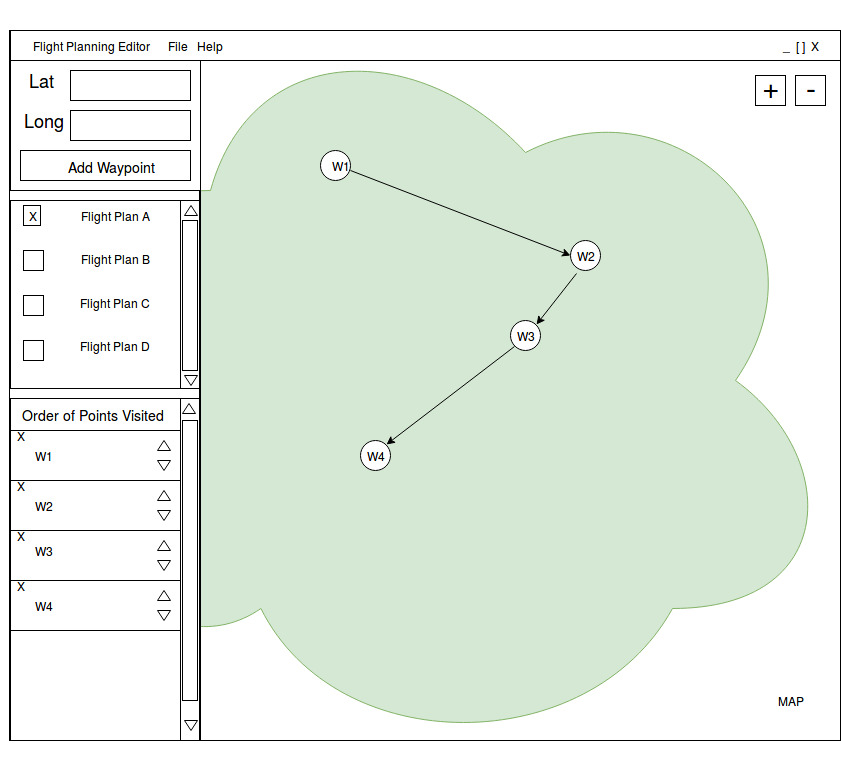
\includegraphics[width=0.95\linewidth]{figs/FlightPlanning_Interface}\caption{Mockup of User Interface}
    \end{figure}
	\subsection{Screen Objects and Actions}
In the above window there are effectively four subsections to the interface. In the upper left corner, where it reads 'Lat', this portion of the interface is where the user can input both the lattitude and longitude coordinates as input into the flight editor. To add these coordinates to the current flight plan, simply click on the 'Add Waypoint' box and the program will create a new point on the map as well as create an addition into the Order of Points Visited section detailed below. \\
Directly below, there will be another section which reads the various flight plans that are currently loaded and their respective names (i.e. Flight Plan A). To distinguish which flight plan the user wants to current edit, that flight plan will have a box which shows an 'X' or is checked to denote that it is currently selected. \\
Underneath the above section, in the lower left corner of the application, there is a section for the order of points visited. In this section there will be a list of all the currently added waypoints named 'W1', 'W2'... Each of these waypoints are listed in order from top to the bottom. To the right of these names there are arrows pointing upwards and downwards, and by clicking on this icon up or down, the user will be able to re-arrange the order in which each point is visited and the application will swap the waypoint boxes in this section, as well as redraw the arrow on the map to reflect the changes made. In the upper left portion of each boxes for the waypoints will be a small box with an 'X' when clicked will delete the waypoint and remove it from the map.\\
The largest portion of the interface will display the map. This section will display the current area that the user has selected by panning and zooming in or out of the map. Inside there will be each of the waypoints listed and arrows denoting the direction of the flight plan. As the user enters a new lattitude and longitude, these waypoints will be refreshed and shown ontop of the map in their respective locations. \\
Also included, however not displayed in the diagram are the file and help pull down menus. Within the file menu, there will be the option to start a new or open an existing flight plan. The ability to save the flight plan, or to export onto the SD card. As well as being able to exit the application. Under the help menu, there will be a tutorial to showcase the basic functionality and an included about page with the company information and the version number of the application.

\appendix
\section{Remove Me!}
\begin{figure}[!ht]
    \centering
    \includegraphics{example-diagram}
\end{figure}
This is an example of adding a diagram with plantuml.
Make sure you have an appropriately named UML file in the plantuml folder,
and just use includegraphics.


% \bibliography{citations}{}
% \bibliographystyle{plain}
\end{document}
